\documentclass[11pt, a4paper]{article}

\usepackage{amsmath, amssymb, titling}
\usepackage[margin=2.5cm]{geometry}
\usepackage[colorlinks=true, linkcolor=black, urlcolor=black, citecolor=black]{hyperref}
\usepackage{graphicx}
\usepackage{caption}
\usepackage{subcaption}
\usepackage{float}
\usepackage{cancel}
\usepackage{fancyhdr, lastpage}
\usepackage{fourier-orns}
\usepackage{xcolor}
\usepackage{nomencl}
\makenomenclature
\usepackage{etoolbox}
\usepackage{ifthen}

\setlength{\headheight}{18.2pt}
\setlength{\nomlabelwidth}{1.5cm}

\renewcommand\maketitlehooka{\null\mbox{}\vfill}
\renewcommand\maketitlehookd{\vfill\null}
\renewcommand{\headrule}{\vspace{-5pt}\hrulefill\raisebox{-2.1pt}{\quad\leafleft\decoone\leafright\quad}\hrulefill}
\newcommand{\parder}[2]{\frac{\partial {#1}}{\partial {#2}}}
\renewcommand\nomgroup[1]{%
  \item[\bfseries
  \ifstrequal{#1}{F}{Far--Away Properties}{%
  \ifstrequal{#1}{N}{Dimensionless Numbers}{%
  \ifstrequal{#1}{M}{Matrices}{%
  \ifstrequal{#1}{D}{Diagonals}{%
  \ifstrequal{#1}{V}{Vectors}{%
  \ifstrequal{#1}{P}{Normalized Average Properties}{}}}}}}
]}

\title{Computational Fluid Dynamics \\ HW2}
\author{Almog Dobrescu\\\\ID 214254252}

\pagestyle{fancy}
\cfoot{Page \thepage\ of \pageref{LastPage}}

\begin{document}

\pagestyle{empty}
\maketitle
\thispagestyle{empty}
\newpage

\tableofcontents
\vfil
\listoffigures
\newpage

\printnomenclature
\newpage

\pagestyle{fancy}
\pagenumbering{arabic}
\setcounter{page}{1}
\section{Problem Definition}
\subsection{Governing Equations}
Consider the one-dimensional Navier-Stokes Equations:
\begin{equation}
    \frac{\partial Q}{\partial t}+\frac{\partial E}{\partial x}=\frac{\partial E_\nu}{\partial x}
\end{equation}
\nomenclature[V]{$Q$}{conservation state space vector}
\nomenclature{$t$}{time}
\nomenclature[V]{$E$}{inviscid convective vector}
\nomenclature[V]{$E_\nu$}{viscous convective vector}
\nomenclature{$x$}{spatial coordinate}
Where:
\begin{equation}
    \begin{array}{c}
        \begin{matrix}
            Q=\begin{pmatrix}
                \rho \\\\
                \rho u \\\\
                e
            \end{pmatrix}, & E=\begin{pmatrix}
                \rho u \\\\
                p+\rho u^2 \\\\
                \left(e+p\right)u
            \end{pmatrix}, & E_\nu=\begin{pmatrix}
                0 \\\\
                \tau_{xx} \\\\
                u\tau_{xx}-q_x
            \end{pmatrix}=\begin{pmatrix}
                0 \\\\
                \displaystyle\frac{4}{3}\mu\frac{\partial u}{\partial x} \\\\
                \displaystyle\frac{4}{3}\mu u\frac{\partial u}{\partial x}+\kappa\frac{\partial T}{\partial x}
            \end{pmatrix}
        \end{matrix} \\\\
        \begin{matrix}
            \displaystyle p=\left(\gamma-1\right)\left(e-\frac{1}{2}\rho u^2\right), & \displaystyle T=\frac{p}{\rho R}, \\\\
            \displaystyle\mu=1.458\cdot10^{-6}\frac{T^{\frac{3}{2}}}{T+110.4}, & \displaystyle\kappa=2.495\cdot10^{-3}\frac{T^{\frac{3}{2}}}{T+194}
        \end{matrix} \\\\
        \begin{matrix}
            R=c_p-c_v, & \displaystyle\gamma=\frac{c_p}{c_v}
        \end{matrix}
    \end{array}
    \label{eq: definitions}
    \nomenclature{$\rho$}{fluid density}
    \nomenclature{$u$}{fluid velocity}
    \nomenclature{$e$}{total energy}
    \nomenclature{$p$}{pressure}
    \nomenclature{$\gamma$}{ratio of specific heats}
    \nomenclature{$T$}{temperature}
    \nomenclature{$R$}{gas constant}
    \nomenclature{$\mu$}{coefficient of viscosity}
    \nomenclature{$\kappa$}{coefficient of thermal conductivity}
    \nomenclature{$c_p$}{constant specific heat capacity for a constant pressure}
    \nomenclature{$c_v$}{constant specific heat capacity for a constant volume}
\end{equation}
The constants are:
\begin{itemize}
    \item $\gamma=1.4$ for air under standard atmospheric conditions
    \item $R=287.0$ for air
\end{itemize}

\subsection{Physical Domain}
The physical domain is a tube extended between $x=0.2$ and $x=1.0$. At both ends there are impermeable walls.

\subsection{Initial Conditions}
The initial conditions are shown in Fig.\ref{fig: initial conditions}:
\begin{figure}[H]
    \centering
    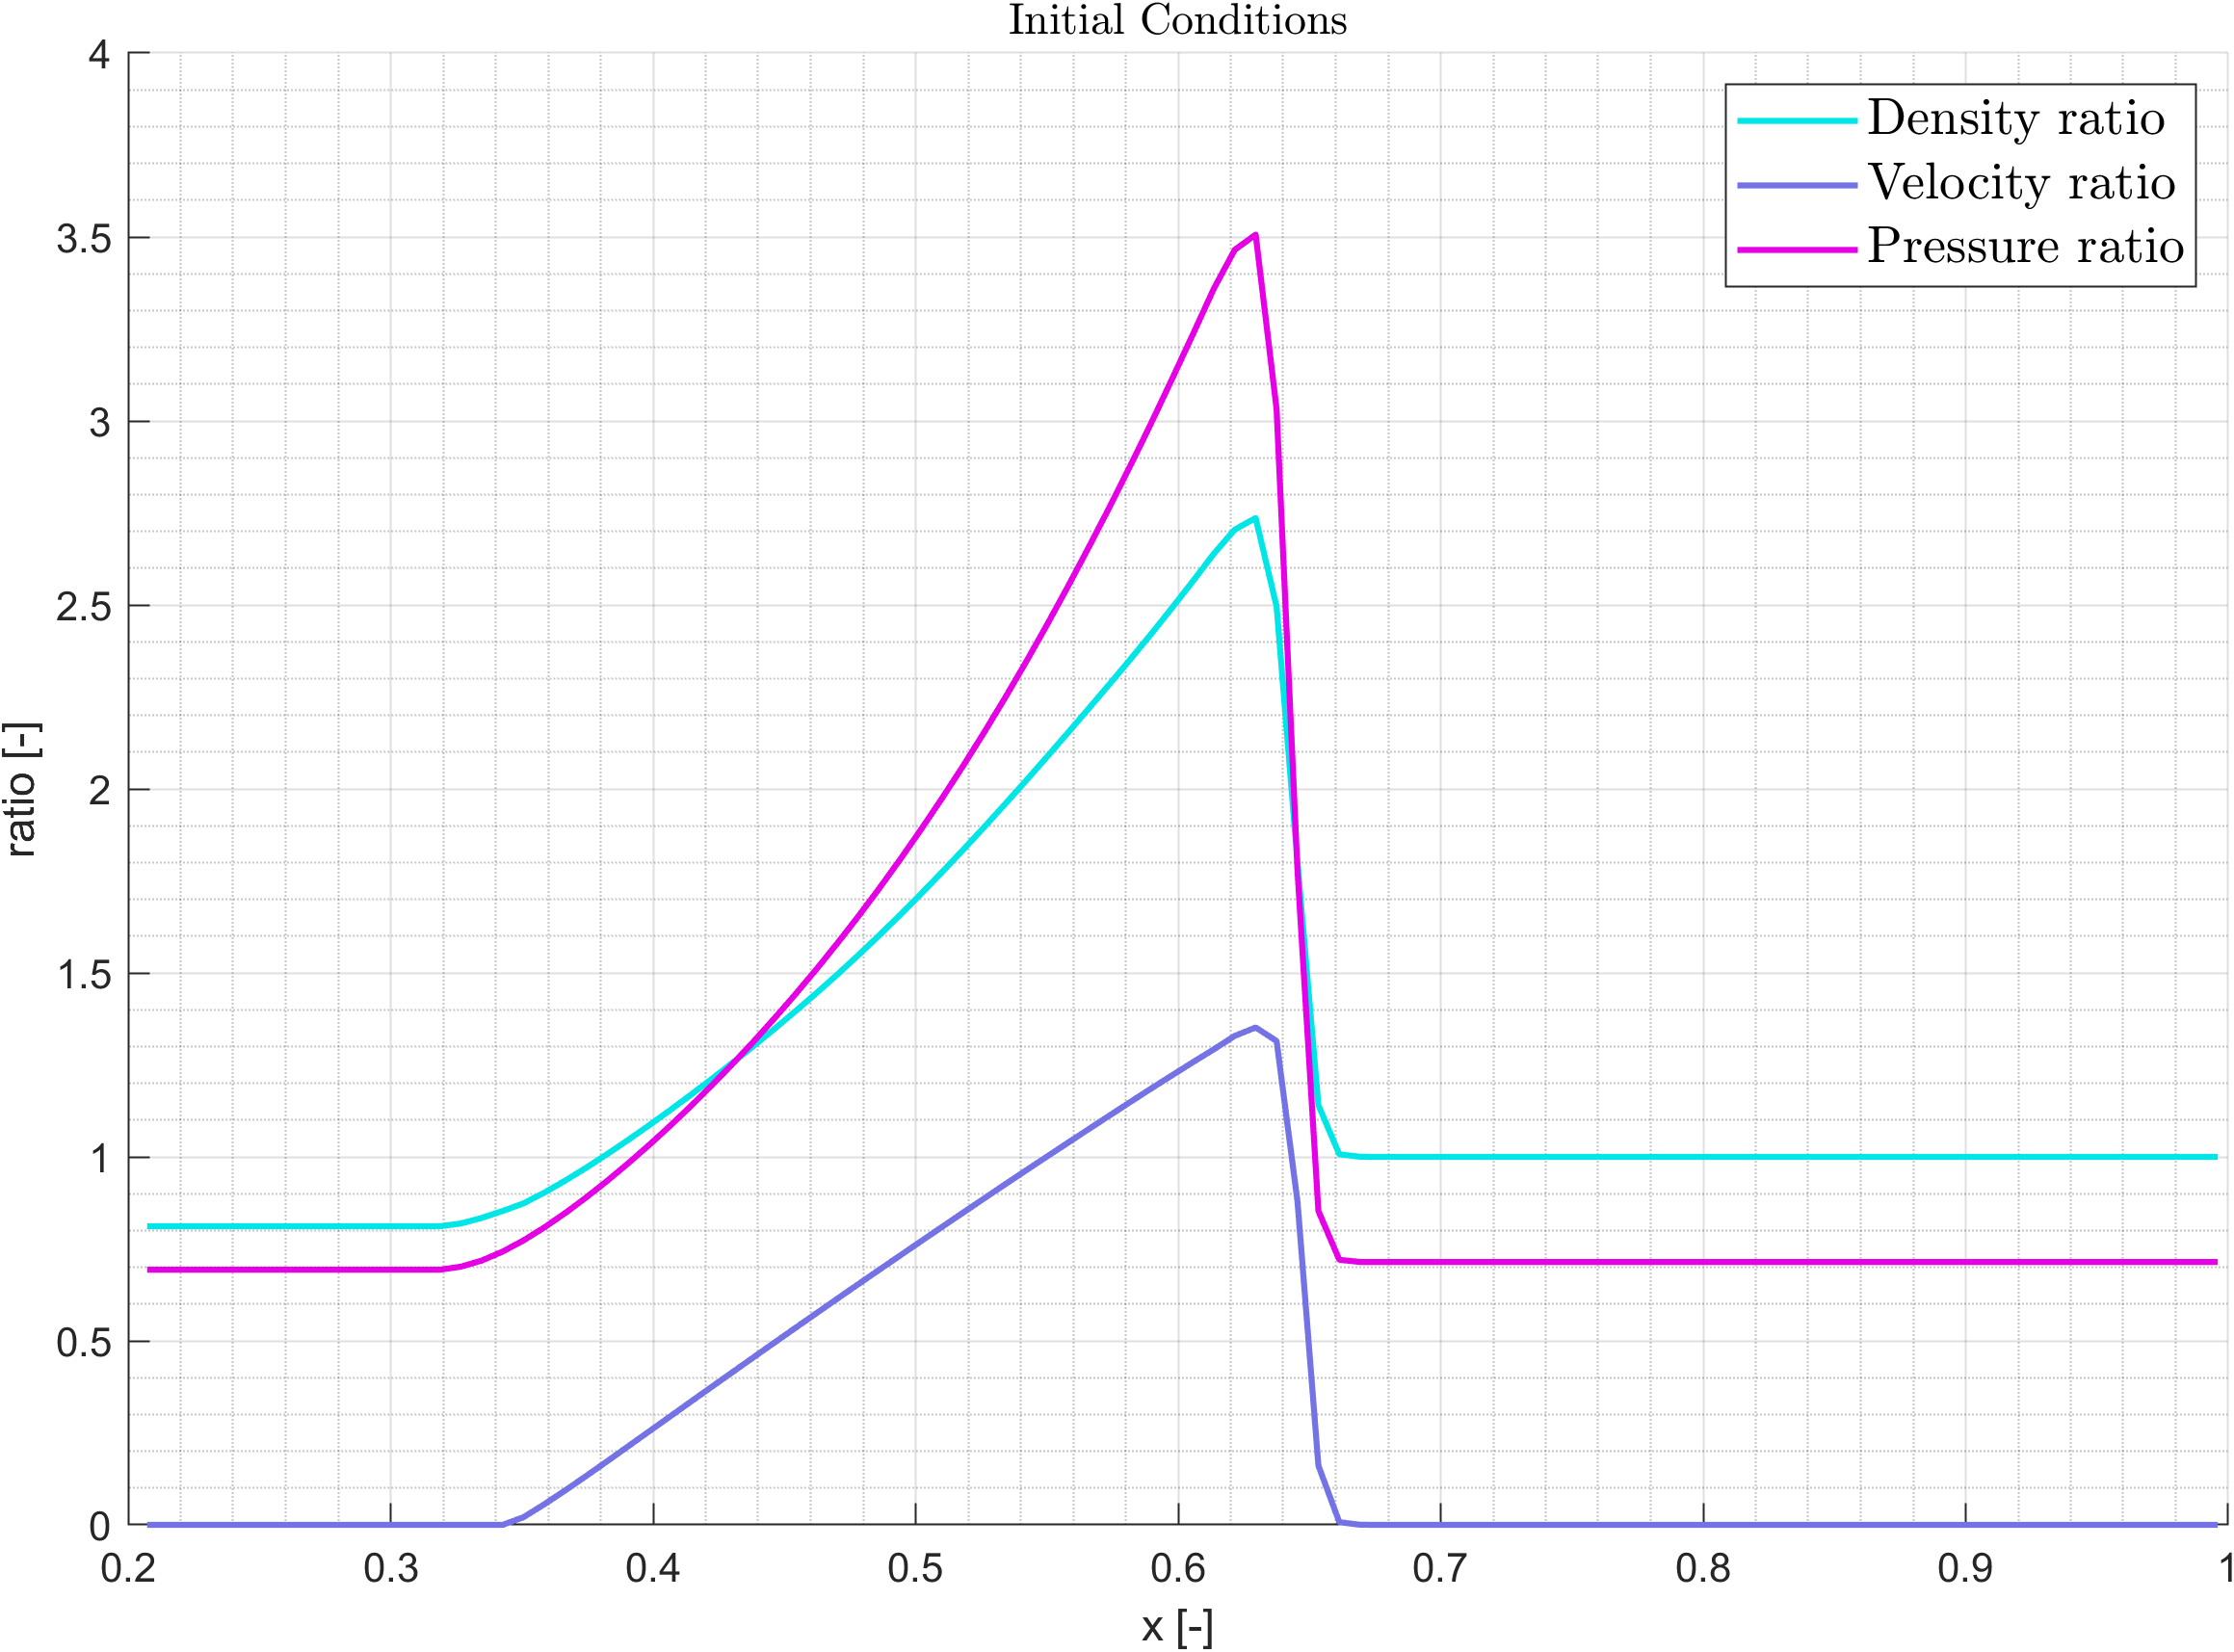
\includegraphics[width=0.4\textwidth]{images/Initial Conditions.png}
    \caption{Initial conditions}
    \label{fig: initial conditions}
\end{figure}

\subsection{Boundary Conditions}
On each side of the tube there is an adiabatic, solid wall boundary conditions. 
\begin{table}[H]
    \centering
    \begin{tabular}{cc||ccc||cc}
        $u_{\left(x=0.2\right)}=u_{\left(x=1.0\right)}=0$ &&& $\displaystyle\left.\frac{\partial p}{\partial x}\right|_{x=0.2}=\left.\frac{\partial p}{\partial x}\right|_{x=1.0}=0$ &&& $\displaystyle\left.\frac{\partial T}{\partial x}\right|_{x=0.2}=\left.\frac{\partial T}{\partial x}\right|_{x=1.0}=0$
    \end{tabular}
\end{table}

\section{Normalizing The Navier-Stokes Equations}
Since the initial conditions are normalized, there is a need to normalize the N-S equations. We will use the following normalizations:
\begin{equation}
    \begin{matrix}
        \rho=\rho_\infty\tilde{\rho}, & u=a_\infty\tilde{u}, & p=\gamma p_\infty\tilde{p}, & T=\gamma T_\infty\tilde{T}, & x=L\tilde{x}, & \displaystyle t=\frac{L}{a_\infty}\tilde{t}, & \mu=\mu_\infty\tilde{\mu}, & \kappa=\kappa_\infty\tilde{\kappa}
    \end{matrix}
    \nomenclature[F]{$\rho_\infty$}{density far away}
    \nomenclature[F]{$a_\infty$}{speed of sound far away}
    \nomenclature[F]{$p_\infty$}{pressure far away}
    \nomenclature[F]{$T_\infty$}{temperature far away}
    \nomenclature[F]{$\mu_\infty$}{coefficient of viscosity far away}
    \nomenclature[F]{$\kappa_\infty$}{coefficient of thermal conductivity far away}
\end{equation}
The normalization of the temperature was chosen to cancel out the $\gamma$ in the normalization of the pressure:
\begin{equation}
    \begin{array}{lcl}
        p & = & \rho RT \\
        \gamma p_\infty\tilde{p} & = & \rho_\infty\tilde{\rho}R\gamma T_\infty\tilde{T} \\
        \tilde{p} & = & \tilde{\rho}\tilde{T}
    \end{array}
\end{equation}
The pressure normalization can be written also as:
\begin{equation}
    p=\gamma p_\infty\tilde{p}=\gamma\rho_\infty RT_\infty\tilde{p}=\rho_\infty a_\infty^2\tilde{p}
    \label{eq: normalization for pressure}
\end{equation}
From equations \ref{eq: definitions} and \ref{eq: normalization for pressure} we can derive the normalization for the energy:
\begin{equation}
    \begin{array}{lcl}
        e & = & \displaystyle\frac{p}{\gamma-1}+\frac{1}{2}\rho u^2 \\\\
        e & = & \displaystyle\frac{\rho_\infty a_\infty^2\tilde{p}}{\gamma-1}+\frac{1}{2}\rho_\infty\tilde{\rho}a_\infty^2\tilde{a}^2 \\\\
        e & = & \displaystyle \rho_\infty a_\infty^2\left(\frac{\tilde{p}}{\gamma-1}+\frac{1}{2}\tilde{\rho}\tilde{a}^2\right) \\\\
        e & = & \rho_\infty a_\infty^2\tilde{e}
    \end{array}
\end{equation}
The normalizations for $\mu$ and $\kappa$ are there for:
\begin{equation}
    \begin{array}{c}
        \begin{array}{lcl}
            \tilde{\mu} & = & \displaystyle\frac{\mu}{\mu_\infty}=\frac{\displaystyle1.458\cdot10^{-6}\frac{\left(\gamma T_\infty\tilde{T}\right)^{\frac{3}{2}}}{\gamma T_\infty\tilde{T}+110.4}}{\displaystyle1.458\cdot10^{-6}\frac{T_\infty^{\frac{3}{2}}}{T_\infty+110.4}}=\frac{\displaystyle\left(\gamma\tilde{T}\right)^{\frac{3}{2}}\left(T_\infty+110.4\right)}{\displaystyle\left(\gamma T_\infty\tilde{T}+110.4\right)}
        \end{array} \\\\
        \begin{array}{lcl}
            \tilde{\kappa} & = & \displaystyle\frac{\kappa}{\kappa_\infty}=\frac{\displaystyle\kappa=2.495\cdot10^{-3}\frac{\left(\gamma T_\infty\tilde{T}\right)^{\frac{3}{2}}}{\gamma T_\infty\tilde{T}+194}}{\displaystyle\kappa=2.495\cdot10^{-3}\frac{T_\infty^{\frac{3}{2}}}{T_\infty+194}}=\frac{\displaystyle\left(\gamma\tilde{T}\right)^{\frac{3}{2}}\left(T_\infty+194\right)}{\displaystyle\left(\gamma T_\infty\tilde{T}+194\right)}
        \end{array}
    \end{array}
\end{equation}
After substituting the normalizations in the N-S equations we get:
\begin{equation}
    \parder{}{\displaystyle\frac{L}{a_\infty}\tilde{t}}\begin{pmatrix}
        \rho_\infty\tilde{\rho} \\\\
        \rho_\infty a_\infty\tilde{\rho}\tilde{u} \\\\
        \rho_\infty a_\infty^2\tilde{e}
    \end{pmatrix}+\parder{}{L\tilde{x}}\begin{pmatrix}
        \rho_\infty a_\infty\tilde{\rho}\tilde{u} \\\\
        \rho_\infty a_\infty^2\tilde{p}+\rho_\infty a_\infty^2\tilde{\rho}\tilde{u}^2 \\\\
        \rho_\infty a_\infty^3\left(\tilde{e}+\tilde{p}\right)\tilde{u}
    \end{pmatrix}=\parder{}{L\tilde{x}}\begin{pmatrix}
        0 \\\\
        \displaystyle\frac{4}{3}\mu_\infty a_\infty\tilde{\mu} \parder{\tilde{u}}{L\tilde{x}} \\\\
        \displaystyle\frac{4}{3}\mu_\infty a_\infty^2\tilde{\mu}\tilde{u}\parder{\tilde{u}}{L\tilde{x}}+\frac{\kappa_\infty a_\infty^2}{R}\tilde{\kappa}\parder{\tilde{T}}{L\tilde{x}}
    \end{pmatrix}
\end{equation}
Rearranging:
\begin{equation}
    \frac{\rho_\infty a_\infty}{L}\parder{}{\tilde{t}}\begin{pmatrix}
        \tilde{\rho} \\\\
        a_\infty\tilde{\rho}\tilde{u} \\\\
        a_\infty^2\tilde{e}
    \end{pmatrix}+\frac{\rho_\infty a_\infty}{L}\parder{}{\tilde{x}}\begin{pmatrix}
        \tilde{\rho}\tilde{u} \\\\
        a_\infty\tilde{p}+a_\infty\tilde{\rho}\tilde{u}^2 \\\\
        a_\infty^2\left(\tilde{e}+\tilde{p}\right)\tilde{u}
    \end{pmatrix}=\frac{\mu_\infty}{L^2}\parder{}{\tilde{x}}\begin{pmatrix}
        0 \\\\
        \displaystyle\frac{4}{3}a_\infty\tilde{\mu} \parder{\tilde{u}}{\tilde{x}} \\\\
        \displaystyle\frac{4}{3}a_\infty^2\tilde{\mu}\tilde{u}\parder{\tilde{u}}{\tilde{x}}+\frac{\kappa_\infty a_\infty^2}{\mu_\infty R}\tilde{\kappa}\parder{\tilde{T}}{\tilde{x}}
    \end{pmatrix}
\end{equation}
Dividing the second equation by $a_\infty$, the third equation by $a_\infty^2$, and the whole set of equations by $\displaystyle\frac{\rho_\infty a_\infty}{L}$ we get:
\begin{equation}
    \parder{}{\tilde{t}}\begin{pmatrix}
        \tilde{\rho} \\\\
        \tilde{\rho}\tilde{u} \\\\
        \tilde{e}
    \end{pmatrix}+\parder{}{\tilde{x}}\begin{pmatrix}
        \tilde{\rho}\tilde{u} \\\\
        \tilde{p}+\tilde{\rho}\tilde{u}^2 \\\\
        \left(\tilde{e}+\tilde{p}\right)\tilde{u}
    \end{pmatrix}=\frac{\mu_\infty}{L\rho_\infty a_\infty}\parder{}{\tilde{x}}\begin{pmatrix}
        0 \\\\
        \displaystyle\frac{4}{3}\tilde{\mu} \parder{\tilde{u}}{\tilde{x}} \\\\
        \displaystyle\frac{4}{3}\tilde{\mu}\tilde{u}\parder{\tilde{u}}{\tilde{x}}+\frac{\kappa_\infty}{\mu_\infty R}\tilde{\kappa}\parder{\tilde{T}}{\tilde{x}}
    \end{pmatrix}
\end{equation}
The Reynolds number and the mach number far away are defined as:
\begin{equation}
    \begin{array}{c}
        \begin{matrix}
            \displaystyle M_\infty=\frac{u_\infty}{a_\infty} & \displaystyle Re_{L\infty}=\frac{\rho_\infty u_\infty L}{\mu_\infty}
        \end{matrix} \\
        \Downarrow \\
        \displaystyle \frac{\mu_\infty}{L\rho_\infty a_\infty}=\frac{M_\infty}{Re_{L\infty}}
    \end{array}
    \nomenclature[F]{$M_\infty$}{mach number far away}
    \nomenclature[N]{$Re_{L\infty}$}{Reynolds number with respect to L far away}
\end{equation}
The Prandtl number far away is defined as:
\begin{equation}
    \begin{array}{c}
        \displaystyle Pr_\infty=\frac{c_p\mu_\infty}{\kappa_\infty} \\
        \Downarrow \\
        \displaystyle\frac{\kappa_\infty}{\mu_\infty R}=\frac{c_p}{Pr_\infty \left(c_p-c_v\right)}=\frac{\gamma}{Pr_\infty\left(\gamma-1\right)}
    \end{array}
    \nomenclature[N]{$Pr_\infty$}{Prandtl number far away}
\end{equation}
Substituting into the normalized N-S equations:
\begin{equation}
    \parder{\tilde{Q}}{\tilde{t}}+\parder{\tilde{E}}{\tilde{x}}=\frac{M_\infty}{Re_{L\infty}}\parder{\tilde{E}_\nu}{\tilde{x}}
\end{equation}
Where:
\begin{equation}
    \begin{matrix}
        \tilde{Q}=\begin{pmatrix}
        \tilde{\rho} \\\\
        \tilde{\rho}\tilde{u} \\\\
        \tilde{e}
        \end{pmatrix}, & \tilde{E}=\begin{pmatrix}
        \tilde{\rho}\tilde{u} \\\\
        \tilde{p}+\tilde{\rho}\tilde{u}^2 \\\\
        \left(\tilde{e}+\tilde{p}\right)\tilde{u}
        \end{pmatrix}, & \tilde{E_\nu}=\begin{pmatrix}
        0 \\\\
        \displaystyle\frac{4}{3}\tilde{\mu} \parder{\tilde{u}}{\tilde{x}} \\\\
        \displaystyle\frac{4}{3}\tilde{\mu}\tilde{u}\parder{\tilde{u}}{\tilde{x}}+\frac{\gamma}{Pr_\infty\left(\gamma-1\right)}\tilde{\kappa}\parder{\tilde{T}}{\tilde{x}}
        \end{pmatrix}
    \end{matrix}
\end{equation}
The normalized Navier-Stokes equations are:
\begin{equation}
    \parder{\tilde{Q}}{\tilde{t}}+\parder{\tilde{E}}{\tilde{x}}=\frac{M_\infty}{Re_{L\infty}}\parder{\tilde{V}_1}{\tilde{x}}
    \label{eq: normalized N-S}
\end{equation}
Where:
\begin{equation*}
    \tilde{V}_1=\tilde{V}_{1\left(\tilde{Q},\tilde{Q}_x\right)}=\tilde{E}_\nu
\end{equation*}

\section{The Computational Domain}
\subsection{Discretization}
The physical domain $\left[x_I,x_F\right]$ is discretized into N equispaced cells. The size of each cell is there for:
\nomenclature{$x_I$}{x coordinate of the start of the domain}
\nomenclature{$x_F$}{x coordinate of the end of the domain}
\begin{equation}
    \Delta x=\frac{x_F-x_I}{N}=\frac{L}{N}
    \nomenclature{$\Delta x$}{size of each cell in the domain}
    \nomenclature{$L$}{characteristic length}
\end{equation}
so the x coordinate of the i-th cell $x_i$ is:
\nomenclature{$x_i$}{x coordinate of the i-th cell}
\begin{equation}
    \begin{matrix}
        \displaystyle x_i=x_I+\frac{1}{2}\Delta x+\Delta x\cdot\left(i-1\right) && \text{when starting from $i=1$}
    \end{matrix}
\end{equation}

\subsection{Boundary Conditions}
In order to set the boundary conditions on the edge faces we will define ghost cells that will be calculated as follows:
\begin{equation}
    \begin{array}{lcl}
        u_{\left(i=0\right)} &=& -u_{\left(i=1\right)} \\
        u_{\left(i=N+1\right)} &=& -u_{\left(i=N\right)}
    \end{array}
    \label{eq: velocity boundary}
\end{equation}
in order to maintain velocity zero on the boundary and like so:
\begin{equation}
    \begin{array}{lcl}
        T_{\left(i=0\right)} &=& T_{\left(i=1\right)} \\
        T_{\left(i=N+1\right)} &=& T_{\left(i=N\right)}
    \end{array}
    \label{eq: temp boundary}
\end{equation}
in order to maintain adiabatic boundary conditions.
Since the gradient of the pressure on the wall is zero, we get:
\begin{equation}
    \begin{array}{lcl}
        p_{\left(i=0\right)} &=& p_{\left(i=1\right)} \\
        p_{\left(i=N+1\right)} &=& p_{\left(i=N\right)}
    \end{array}
    \label{eq: pressure boundary}
\end{equation}
From equations \ref{eq: definitions}, \ref{eq: temp boundary}, and \ref{eq: pressure boundary} we can conclude:
\begin{equation}
    \begin{array}{lcl}
        \rho_{\left(i=0\right)} &=& \rho_{\left(i=1\right)} \\
        \rho_{\left(i=N+1\right)} &=& \rho_{\left(i=N\right)}
    \end{array}
    \label{eq: density boundary}
\end{equation}
and from equations \ref{eq: definitions}, \ref{eq: velocity boundary}, \ref{eq: pressure boundary}, and \ref{eq: density boundary} we can conclude:
\begin{equation}
    \begin{array}{lcl}
        e_{\left(i=0\right)} &=& e_{\left(i=1\right)} \\
        e_{\left(i=N+1\right)} &=& e_{\left(i=N\right)}
    \end{array}
    \label{eq: energy boundary}
\end{equation}
\newpage

\section{The Numerical Schemes}
\subsection{Jacobian Matrices of The Navier-Stokes Equations}
We can rewrite Eq.\ref{eq: normalized N-S} as:
\begin{equation}
    \begin{array}{lcl}
        \displaystyle\parder{\tilde{Q}}{\tilde{t}} & = & \displaystyle-\parder{\tilde{E}}{\tilde{x}}-\frac{M_\infty}{Re_{L\infty}}\parder{\tilde{V}_1}{\tilde{x}} \\\\
        \displaystyle\parder{\tilde{Q}}{\tilde{t}} & = & \displaystyle-\underbrace{\parder{\tilde{E}}{\tilde{Q}}}_{\tilde{A}}\parder{\tilde{Q}}{\tilde{x}}-\frac{M_\infty}{Re_{L\infty}}\left(\underbrace{\parder{\tilde{V}_1}{\tilde{Q}}}_{\tilde{P}}\parder{\tilde{Q}}{\tilde{x}}+\underbrace{\parder{\tilde{V}_1}{\tilde{Q}_x}}_{\tilde{R}}\parder{\tilde{Q}_x}{\tilde{x}}\right)
    \end{array}
    \label{eq: chain rule}
\end{equation}
Where:
\begin{equation}
    \begin{array}{ccl}
        \tilde{A} & = & \begin{pmatrix}
            0 & 1 & 0 \\
            \displaystyle\frac{\gamma-3}{2}\tilde{u}^2 & \left(3-\gamma\right)\tilde{u} & \gamma-1 \\
            \displaystyle-\frac{\gamma\tilde{e}\tilde{u}}{\tilde{\rho}}-\left(\gamma-1\right)\tilde{u}^3 & \displaystyle\frac{\gamma\tilde{e}}{\tilde{\rho}}-\frac{3\left(\gamma-1\right)\tilde{u}^2}{2} & \gamma\tilde{u}
        \end{pmatrix} \\\\
        \tilde{P}-\tilde{R}_x & = & \displaystyle-\frac{1}{\rho}\begin{pmatrix}
            0 & 0 & 0 \\\\
            \displaystyle-\tilde{u}\left(\frac{4}{3}\tilde{\mu}\right)_x & \displaystyle\left(\frac{4}{3}\tilde{\mu}\right)_x & 0 \\\\
            \displaystyle-\tilde{u}^2\left(\frac{4}{3}\tilde{\mu}\right)_x & \displaystyle\tilde{u}\left(\frac{4}{3}\tilde{\mu}\right)_x & 0
        \end{pmatrix} \\\\
        \tilde{R} & = & \displaystyle-\frac{1}{\rho}\begin{pmatrix}
            0 & 0 & 0 \\\\
            \displaystyle\frac{4}{3}\tilde{u}\tilde{\mu} & \displaystyle-\frac{4}{3}\tilde{\mu} & 0 \\\\
            \displaystyle\left(\frac{4}{3}\tilde{\mu}-\textcolor{blue}{\alpha}\frac{\tilde{\kappa}}{c_v}\right)\tilde{u}^2+\textcolor{blue}{\alpha}\frac{\tilde{\kappa}}{c_v}\frac{\tilde{e}}{\tilde{\rho}} & \displaystyle-\left(\frac{4}{3}\tilde{\mu}-\textcolor{blue}{\alpha}\frac{\tilde{\kappa}}{c_v}\right)\tilde{u} & \displaystyle-\textcolor{blue}{\alpha}\frac{\tilde{\kappa}}{c_v}
        \end{pmatrix}
    \end{array}
    \label{eq: A P R}
\end{equation}
and $\textcolor{blue}{\alpha}$ is: $$\textcolor{blue}{\alpha=\frac{\gamma}{Pr_\infty\left(\gamma-1\right)}}$$
\nomenclature[M]{$\tilde{A}$}{normalized jacobian matrix of E w.r.t. Q}
\nomenclature[M]{$\tilde{P}$}{normalized jacobian matrix of $E_\nu$ w.r.t. Q}
\nomenclature[M]{$\tilde{R}$}{normalized jacobian matrix of $E_\nu$ w.r.t. $Q_x$}

\subsection{FVS -- First Order Explicit Steger-Warming}
Since the inviscid N-S equations (Euler equations) is a hyperbolic system of equations, the A matrix (from Eq.\ref{eq: A P R}) is a diagonalizable matrix and can be written as:
\begin{equation}
    \begin{array}{c}
        \tilde{A}=\tilde{T}\tilde{\Lambda}\tilde{T}^{-1} \\
        \tilde{T}=\begin{pmatrix}
            1 & \displaystyle\frac{\tilde{\rho}}{2\tilde{a}} & \displaystyle-\frac{\tilde{\rho}}{2\tilde{a}} \\\\
            \tilde{u} & \displaystyle\frac{\tilde{\rho}}{2\tilde{a}}\left(\tilde{u}+\tilde{a}\right) & \displaystyle-\frac{\tilde{\rho}}{2\tilde{a}}\left(\tilde{u}-\tilde{a}\right) \\\\
            \displaystyle\frac{\tilde{u}^2}{2} & \displaystyle\frac{\tilde{\rho}}{2\tilde{a}}\left(\frac{\tilde{u}^2}{2}+\tilde{u}\tilde{a}+\frac{\tilde{a}^2}{\gamma-1}\right) & \displaystyle-\frac{\tilde{\rho}}{2\tilde{a}}\left(\frac{\tilde{u}^2}{2}-\tilde{u}\tilde{a}+\frac{\tilde{a}^2}{\gamma-1}\right)
        \end{pmatrix} \\\\
        \tilde{\Lambda}=\begin{pmatrix}
            \tilde{u} & 0 & 0 \\
            0 & \tilde{u}+\tilde{a} & 0 \\
            0 & 0 & \tilde{u}-\tilde{a}
        \end{pmatrix} \\\\
        \tilde{T}^{-1}=\begin{pmatrix}
            \displaystyle1-\frac{\gamma-1}{2}\frac{\tilde{u}^2}{\tilde{a}^2} & \displaystyle\left(\gamma-1\right)\frac{\tilde{u}^2}{\tilde{a}^2} & \displaystyle-\frac{\gamma-1}{\tilde{a}^2} \\\\
            \displaystyle\frac{1}{\tilde{\rho}\tilde{a}}\left(\left(\gamma-1\right)\tilde{u}^2-\tilde{u}\tilde{a}\right) & \displaystyle\frac{1}{\tilde{\rho}\tilde{a}}\left(\tilde{a}-\left(\gamma-1\right)\tilde{u}\right) & \displaystyle\frac{\gamma-1}{\tilde{\rho}\tilde{a}} \\\\
            \displaystyle-\frac{1}{\tilde{\rho}\tilde{a}}\left(\left(\gamma-1\right)\tilde{u}^2+\tilde{u}\tilde{a}\right) & \displaystyle\frac{1}{\tilde{\rho}\tilde{a}}\left(\tilde{a}+\left(\gamma-1\right)\tilde{u}\right) & \displaystyle-\frac{\gamma-1}{\tilde{\rho}\tilde{a}}
        \end{pmatrix}
    \end{array}
    \nomenclature[M]{$\tilde{T}$}{normalized eigenvectors matrix}
    \nomenclature[M]{$\tilde{\Lambda}$}{normalized eigenvalues matrix}
    \label{eq: T Labmda T^-1}
\end{equation}
Where:
\begin{equation*}
    \tilde{a}=\sqrt{\frac{\gamma\tilde{p}}{\tilde{\rho}}}
\end{equation*}
Let the $\tilde{\Lambda}^\pm$ matrix be defined as:
\begin{equation}
    \tilde{\Lambda}^\pm=\begin{pmatrix}
        \displaystyle\frac{\tilde{u}\pm\left|\tilde{u}\right|}{2} & 0 & 0 \\
        0 & \displaystyle\frac{\tilde{u}+\tilde{a}\pm\left|\tilde{u}+\tilde{a}\right|}{2} & 0 \\
        0 & 0 & \displaystyle\frac{\tilde{u}-\tilde{a}\pm\left|\tilde{u}-\tilde{a}\right|}{2}
    \end{pmatrix}
\end{equation}
Where the matrix $\tilde{\Lambda}^+$ contains only positive eigenvalues and the matrix $\tilde{\Lambda}^-$ contains only negative eigenvalues. As in Roe's scheme, one can define:
\begin{equation}
    \begin{matrix}
        \begin{array}{ccl}
            \tilde{A}^+ & \triangleq & \tilde{T}\tilde{\Lambda}^+\tilde{T}^{-1} \\
            \tilde{A}^- & \triangleq & \tilde{T}\tilde{\Lambda}^-\tilde{T}^{-1}
        \end{array} & \Rightarrow & \begin{array}{ccl}
            \tilde{A} & = & \tilde{A}^++\tilde{A}^- \\
            \left|\tilde{A}\right| & \triangleq & \tilde{A}^+-\tilde{A}^-
        \end{array}
    \end{matrix}
\end{equation}
Assuming a perfect gas, the flux vector $\tilde{E}_{\left(Q\right)}$ is a homogeneous function of degree one in $\tilde{Q}$, meaning:$$\forall\alpha\ \ \ \ \tilde{E}_{\left(\alpha \tilde{Q}\right)}=\alpha \tilde{E}_{\left(\tilde{Q}\right)}$$The homogeneity allows to rewrite the flux vector $\tilde{E}$ using Eq.\ref{eq: chain rule} as:
\begin{equation}
    \tilde{E}=\tilde{A}\tilde{Q}=\left(\tilde{A}^++\tilde{A}^-\right)\tilde{Q}=\underbrace{\tilde{A}^+\tilde{Q}}_{\displaystyle\tilde{E}^+}+\underbrace{\tilde{A}^-\tilde{Q}}_{\displaystyle\tilde{E}^-}=\tilde{E}^++\tilde{E}^-
    \label{eq: E vector splitting}
\end{equation} 
There is a discontinuity and deference between $\tilde{E}^+,\tilde{E}^-$.
% There is a discontinuities and deference between $\tilde{E}^+,\tilde{E}^-$ for example:
% \begin{equation}
%     \begin{matrix}
%         \tilde{E}^+_1=\left\{\begin{array}{lc}
%             0 & M\le-1 \\\\
%             \displaystyle\frac{\tilde{\rho} \tilde{a}}{2\gamma}\left(M+1\right) & -1\le M\le0 \\\\
%             \displaystyle\frac{\tilde{\rho} \tilde{a}}{2\gamma}\left(\left(2\gamma-1\right)M+1\right) & 0\le M\le1 \\\\
%             \tilde{E}_1 & 1\le M
%         \end{array}\right. & \tilde{E}^-_1=\left\{\begin{array}{lc}
%             \tilde{E}_1 & M\le-1 \\\\
%             \displaystyle\frac{\tilde{\rho} \tilde{a}}{2\gamma}\left(\left(2\gamma-1\right)M-1\right) & -1\le M\le0 \\\\
%             \displaystyle\frac{\tilde{\rho} \tilde{a}}{2\gamma}\left(M-1\right) & 0\le M\le1 \\\\
%             0 & 1\le M
%         \end{array}\right.
%     \end{matrix}
% \end{equation}
To eliminate the discontinuities and guarantee a smooth transition through critical points (sonic points or stagnation points), a blending function is introduced together with a blending parameter $\varepsilon$. An appropriate choice of the blending parameter has to be chosen.
\begin{equation}
    \begin{matrix}
        \begin{array}{lcl}
            \tilde{\lambda}^+ & = & \displaystyle\frac{\tilde{\lambda}+\left|\tilde{\lambda}\right|}{2} \\\\
            \tilde{\lambda}^- & = & \displaystyle\frac{\tilde{\lambda}-\left|\tilde{\lambda}\right|}{2}
        \end{array} & \Rightarrow & \begin{array}{lcl}
            \tilde{\lambda}^{+'} & = & \displaystyle\frac{\tilde{\lambda}+\sqrt{\tilde{\lambda}^2+\varepsilon^2}}{2} \\\\
            \tilde{\lambda}^{-'} & = & \displaystyle\frac{\tilde{\lambda}-\sqrt{\tilde{\lambda}^2+\varepsilon^2}}{2}
        \end{array}
    \end{matrix}
\end{equation}
Rewriting the conservation law form of the N-S equations Eq.\ref{eq: normalized N-S} using Eq.\ref{eq: E vector splitting}:
\begin{equation}
    \parder{\tilde{Q}}{\tilde{t}}=-\parder{\tilde{E}^+}{\tilde{x}}-\parder{\tilde{E}^-}{\tilde{x}}+\frac{M_\infty}{Re_{L\infty}}\parder{\tilde{V}_1}{\tilde{x}}
\end{equation}
A simple, explicit, first order (in space and time) scheme in delta form is obtained using:
\begin{equation}
    \Delta\tilde{Q}_i^n=\displaystyle-\frac{\Delta\tilde{t}}{\Delta\tilde{x}}\left(\nabla\tilde{E}_i^{+n}+\Delta\tilde{E}_i^{-n}-\frac{M_\infty}{Re_{L\infty}}\delta\tilde{V}_{1,i}^{n}\right)
    \label{eq: explicit S-W delta form}
    \nomenclature{$\Delta\tilde{t}$}{normalized step size in time}
    \nomenclature{$\Delta\tilde{x}$}{normalized step size in space}
\end{equation}
And advancing the solution by:
\begin{equation}
    \tilde{Q}_i^{n+1}=\Delta\tilde{Q}_i^n+\tilde{Q}_i^n
\end{equation} 

\subsubsection{Finite Volume Formulation}
Rearranging Eq.\ref{eq: explicit S-W delta form} using the finite volume notation:
\begin{equation}
    \begin{array}{lcl}
        \Delta\tilde{Q}_i^n & = & \displaystyle-\frac{\Delta\tilde{t}}{\Delta\tilde{x}}\left(\tilde{E}_i^{+n}-\tilde{E}_{i-1}^{+n}+\tilde{E}_{i+1}^{-n}-\tilde{E}_i^{-n}-\frac{M_\infty}{Re_{L\infty}}\left(\tilde{V}_{1,i+\frac{1}{2}}^{n}-\tilde{V}_{1,i-\frac{1}{2}}^{n}\right)\right) \\\\
        \Delta\tilde{Q}_i^n & = & \displaystyle-\frac{\Delta\tilde{t}}{\Delta\tilde{x}}\left(\left(\tilde{E}_i^{+n}+\tilde{E}_{i+1}^{-n}\right)-\left(\tilde{E}_{i-1}^{+n}+\tilde{E}_i^{-n}\right)-\frac{M_\infty}{Re_{L\infty}}\left(\tilde{V}_{1,i+\frac{1}{2}}^{n}-\tilde{V}_{1,i-\frac{1}{2}}^{n}\right)\right)
    \end{array}
\end{equation}
Define:
\begin{equation}
    \begin{array}{lcl}
        \tilde{E}_{i+\frac{1}{2}} & \triangleq & \tilde{E}_i^++E_{i+1}^- \\\\
        & = & \tilde{A}^+_i\tilde{Q}_i+\tilde{A}^-_{i+1}\tilde{Q}_{i+1} \\\\
        & \equiv & \tilde{\tilde{E}}_{i+\frac{1}{2}}
    \end{array}
\end{equation}
Finally we get:
\begin{equation}
    \Delta\tilde{Q}_i^n=-\frac{\Delta\tilde{t}}{\Delta\tilde{x}}\left(\tilde{\tilde{E}}_{i+\frac{1}{2}}^n-\tilde{\tilde{E}}_{i-\frac{1}{2}}^n-\frac{M_\infty}{Re_{L\infty}}\left(\tilde{V}_{1,i+\frac{1}{2}}^{n}-\tilde{V}_{1,i-\frac{1}{2}}^{n}\right)\right)
    \label{eq: finall explicit S-W}
\end{equation}
\subsubsection{Calculating $\tilde{V}_{1,i+\frac{1}{2}}$}
\begin{equation}
    \tilde{V}_{1,i+\frac{1}{2}}=\begin{pmatrix}
        0 \\\\
        \displaystyle\frac{4}{3}\left.\tilde{\mu}\right|_{i+\frac{1}{2}}\left.\parder{\tilde{u}}{\tilde{x}}\right|_{i+\frac{1}{2}} \\\\
        \displaystyle\frac{4}{3}\left.\tilde{\mu}\right|_{i+\frac{1}{2}}\left.\tilde{u}\right|_{i+\frac{1}{2}}\left.\parder{\tilde{u}}{\tilde{x}}\right|_{i+\frac{1}{2}}+\frac{\gamma}{Pr_\infty\left(\gamma-1\right)}\left.\tilde{\kappa}\right|_{i+\frac{1}{2}}\left.\parder{\tilde{T}}{\tilde{x}}\right|_{i+\frac{1}{2}}
        \end{pmatrix}
\end{equation}
Where:
\begin{equation}
    \begin{array}{c}
        \begin{matrix}
            \begin{array}{lcl}
                \displaystyle\left.\parder{\tilde{u}}{\tilde{x}}\right|_{i+\frac{1}{2}} & = & \displaystyle\frac{\tilde{u}_{i+1}-\tilde{u}_i}{\Delta\tilde{x}}, \\\\
                \displaystyle\left.\parder{\tilde{T}}{\tilde{x}}\right|_{i+\frac{1}{2}} & = & \displaystyle\frac{\tilde{T}_{i+1}-\tilde{T}_i}{\Delta\tilde{x}},
            \end{array} \hspace{0.5cm}&\hspace{0.5cm} \begin{array}{lcl}
                \displaystyle\left.\tilde{\mu}\right|_{i+\frac{1}{2}} & = & \displaystyle\frac{\tilde{\mu}_{i+1}+\tilde{\mu}_i}{2} \\\\
                \displaystyle\left.\tilde{\kappa}\right|_{i+\frac{1}{2}} & = & \displaystyle\frac{\tilde{\kappa}_{i+1}+\tilde{\kappa}_i}{2} \\\\
            \end{array}
        \end{matrix}\\\\
        \displaystyle\left.\tilde{u}\right|_{i+\frac{1}{2}}=\frac{\tilde{u}_{i+1}+\tilde{u}_i}{2} \\\\
    \end{array}
\end{equation}

\subsection{FVS -- First Order Implicit Steger-Warming}

\subsubsection{Linearization In Time}
\begin{itemize}
    \item $\tilde{E}_i^{n+1}$ Estimation
        \begin{equation}
            \begin{array}{c}
                \displaystyle\tilde{E}_i^{n+1}=\tilde{E}_i^{n}+\underbrace{\left.\parder{\tilde{E}}{\tilde{Q}}\right|_i^n}_{\displaystyle\tilde{A}_i^n}\Delta\tilde{Q}_i^n+\mathrm{H.O.T} \\\\
                \displaystyle\tilde{E}_i^{n+1}=\tilde{E}_i^{n}+\tilde{A}_i^n\Delta\tilde{Q}_i^n
            \end{array}
        \end{equation}
    \item $\tilde{V_1}_{i}^{n+1}$ Estimation 
        \begin{equation}
            \begin{array}{c}
                \displaystyle\tilde{V}_{1,i}^{n+1}=\tilde{V}_{1,i}^{n}+\underbrace{\left.\parder{\tilde{V}_1}{\tilde{Q}}\right|_i^n}_{\displaystyle\tilde{P}_i^n}\Delta\tilde{Q}_i^n+\underbrace{\left.\parder{\tilde{V}_1}{\tilde{Q}_x}\right|_i^n}_{\displaystyle\tilde{R}_i^n}\Delta\tilde{Q_x}_i^n+\mathrm{H.O.T} \\\\
                \displaystyle\tilde{V}_{1,i}^{n+1}=\tilde{V}_{1,i}^{n}+\tilde{P}_i^n\Delta\tilde{Q}_i^n+\tilde{R}_i^n\Delta\tilde{Q_x}_i^n \\\\
            \end{array}
        \end{equation}
        The difficulty stems from the fact that the solution vector is $\Delta\tilde{Q}$ and not $\Delta\tilde{Q}_x$. This can be solved by a linearization of the term $\Delta\tilde{Q}_x$ which can be conducted using the following relation:
        \begin{equation*}
            \parder{\left(\tilde{R}\Delta\tilde{Q}\right)_i^n}{\tilde{x}}=\parder{\tilde{R}_i^n}{\tilde{x}}\Delta\tilde{Q}_i^n+\tilde{R}_i^n\parder{\Delta\tilde{Q}_i^n}{\tilde{x}}=\parder{\tilde{R}}{\tilde{x}}\Delta\tilde{Q}+\tilde{R}_i^n\Delta\tilde{Q_x}_i^n 
        \end{equation*}
        $$\Downarrow$$
        \begin{equation}
            \displaystyle\tilde{V}_{1,i}^{n+1}=\tilde{V}_{1,i}^{n}+\left(\tilde{P}-\tilde{R_x}\right)_i^n\Delta\tilde{Q}_i^n+\parder{}{\tilde{x}}\left(\tilde{R}\Delta\tilde{Q}\right)_i^n 
        \end{equation}
\end{itemize}

\subsubsection{The Scheme}
The Implicit Steger-Warming scheme starts from:
\begin{equation}
    \begin{array}{lcl}
        \displaystyle\frac{\Delta\tilde{Q}_i^n}{\Delta\tilde{t}} & = & \displaystyle-\parder{\tilde{E}_i^{n+1}}{\tilde{x}}+\frac{M_\infty}{Re_{L\infty}}\parder{\tilde{V}_{1,i}^{n+1}}{\tilde{x}} \\\\
        \displaystyle\Delta\tilde{Q}_i^n & = & \displaystyle-\Delta\tilde{t}\parder{}{\tilde{x}}\left(\tilde{E}_i^{n}+\tilde{A}_i^n\Delta\tilde{Q}_i^n\right)+\Delta\tilde{t}\frac{M_\infty}{Re_{L\infty}}\parder{}{\tilde{x}}\left(\tilde{V}_{1,i}^{n}+\left(\tilde{P}-\tilde{R_x}\right)_i^n\Delta\tilde{Q}_i^n+\parder{}{\tilde{x}}\left(\tilde{R}\Delta\tilde{Q}\right)_i^n\right)
    \end{array}
\end{equation}
Rearranging in delta form:
\begin{equation}
    \begin{array}{c}
        \displaystyle\left(I+\Delta\tilde{t}\left(\parder{}{\tilde{x}}\left[\tilde{A}-\frac{M_\infty}{Re_{L\infty}}\left(\tilde{P}-\tilde{R_x}\right)\right]_i^n-\frac{M_\infty}{Re_{L\infty}}\frac{\partial^2\tilde{R}_i^n}{\partial\tilde{x}^2}\right)\right)\Delta\tilde{Q}_i^n=\mathrm{RHS}_i^n \\\\
        \mathrm{RHS}_i^n=\displaystyle-\Delta\tilde{t}\parder{}{\tilde{x}}\left(\tilde{E}^{+}+\tilde{E}^{-}-\frac{M_\infty}{Re_{L\infty}}\tilde{V}_{1}\right)_i^n
    \end{array}
\end{equation}
\begin{equation}
    \begin{array}{c}
        \displaystyle\left(I+\frac{\Delta\tilde{t}}{\Delta\tilde{x}}\left(\left[\nabla\tilde{A}^{+}+\Delta\tilde{A}^{-}-\frac{M_\infty}{Re_{L\infty}}\frac{D_0}{2}\left(\tilde{P}-\tilde{R_x}\right)\right]_i^n-\frac{M_\infty}{Re_{L\infty}}\frac{\delta^2}{\Delta\tilde{x}}\tilde{R}_i^n\right)\right)\Delta\tilde{Q}_i^n=\mathrm{RHS}_i^n \\\\
        \mathrm{RHS}_i^n=\displaystyle-\frac{\Delta\tilde{t}}{\Delta\tilde{x}}\left(\nabla\tilde{E}^{+}+\Delta\tilde{E}^{-}-\frac{M_\infty}{Re_{L\infty}}\delta\tilde{V}_{1}\right)_i^n
    \end{array}
\end{equation}
Rewrite using the finite volume notation for the inviscid terms like in Eq.\ref{eq: finall explicit S-W}:
\begin{equation}
    \begin{array}{c}
        \displaystyle\left(I+\frac{\Delta\tilde{t}}{\Delta\tilde{x}}\left(\left[\nabla\tilde{A}^{+}+\Delta\tilde{A}^{-}-\frac{M_\infty}{Re_{L\infty}}\frac{D_0}{2}\left(\tilde{P}-\tilde{R_x}\right)\right]_i^n-\frac{M_\infty}{Re_{L\infty}}\frac{\delta^2}{\Delta\tilde{x}}\tilde{R}_i^n\right)\right)\Delta\tilde{Q}_i^n=\mathrm{RHS}_i^n \\\\
        \mathrm{RHS}_i^n=\displaystyle-\frac{\Delta\tilde{t}}{\Delta\tilde{x}}\left(\tilde{\tilde{E}}_{i+\frac{1}{2}}^n-\tilde{\tilde{E}}_{i-\frac{1}{2}}^n-\frac{M_\infty}{Re_{L\infty}}\left(\tilde{V}_{1,i+\frac{1}{2}}^{n}-\tilde{V}_{1,i-\frac{1}{2}}^{n}\right)\right)
    \end{array}
\end{equation}
and opening the delta form on the LHS:
% \begin{equation}
%     \begin{array}{lcl}
%         \mathrm{LHS}_i^n & = & \displaystyle\Delta\tilde{Q}_i^n+\frac{\Delta\tilde{t}}{\Delta\tilde{x}}\left(\nabla\tilde{A}_i^{+n}\Delta\tilde{Q}_i^n+\Delta\tilde{A}_i^{-n}\Delta\tilde{Q}_i^n-\delta\left(\tilde{P}-\tilde{R_x}\right)_i^n\Delta\tilde{Q}_i^n-\frac{\delta^2}{\Delta\tilde{x}}\tilde{R}_i^n\Delta\tilde{Q}_i^n\right) \\\\
%     \end{array}
% \end{equation}
\begin{equation}
    \begingroup\makeatletter\def\f@size{11}\check@mathfonts
    \begin{array}{lcl}
        \mathrm{LHS}_i^n & = & \displaystyle\Delta\tilde{Q}_i^n+\frac{\Delta\tilde{t}}{\Delta\tilde{x}}\left(\nabla\tilde{A}_i^{+n}\Delta\tilde{Q}_i^n+\Delta\tilde{A}_i^{-n}\Delta\tilde{Q}_i^n-\frac{M_\infty}{Re_{L\infty}}\frac{D_0}{2}\left(\tilde{P}-\tilde{R_x}\right)_i^n\Delta\tilde{Q}_i^n-\frac{M_\infty}{Re_{L\infty}}\frac{\delta^2}{\Delta\tilde{x}}\tilde{R}_i^n\Delta\tilde{Q}_i^n\right) \\\\
        & = & \displaystyle\Delta\tilde{Q}_i^n+\frac{\Delta\tilde{t}}{\Delta\tilde{x}}\left(\tilde{A}_i^{+n}\Delta\tilde{Q}_i^n-\tilde{A}_{i-1}^{+n}\Delta\tilde{Q}_{i-1}^n+\tilde{A}_{i+1}^{-n}\Delta\tilde{Q}_{i+1}^n-\tilde{A}_i^{-n}\Delta\tilde{Q}_i^n-\right. \\\\
        & & \displaystyle-\frac{1}{2}\frac{M_\infty}{Re_{L\infty}}\left[\left(\tilde{P}-\tilde{R_x}\right)_{i+1}^n\Delta\tilde{Q}_{i+1}^n-\left(\tilde{P}-\tilde{R_x}\right)_{i-1}^n\Delta\tilde{Q}_{i-1}^n\right]- \\\\
        & & \displaystyle-\left.\frac{1}{\Delta\tilde{x}}\frac{M_\infty}{Re_{L\infty}}\left[\tilde{R}_{i+1}^n\Delta\tilde{Q}_{i+1}^n-2\tilde{R}_i^n\Delta\tilde{Q}_i^n+\tilde{R}_{i-1}^n\Delta\tilde{Q}_{i-1}^n\right]\right) \\\\
        & = & \displaystyle\Theta_i^n\Delta\tilde{Q}_{i-1}^n+\Phi_i^n\Delta\tilde{Q}_i^n+\Psi_i^n\Delta\tilde{Q}_{i+1}^n
    \end{array}
    \endgroup
    \nomenclature[D]{$\Theta$}{lower off-diagonal}
    \nomenclature[D]{$\Phi$}{main diagonal}
    \nomenclature[D]{$\Psi$}{upper off-diagonal}
\end{equation}
Where:
\begin{equation}
    \begin{array}{lcl}
        \Theta_i^n & = & \displaystyle-\frac{\Delta\tilde{t}}{\Delta\tilde{x}}\tilde{A}_{i-1}^{+n}+\frac{\Delta\tilde{t}}{2\Delta\tilde{x}}\frac{M_\infty}{Re_{L\infty}}\left(\tilde{P}-\tilde{R_x}\right)_{i-1}^n-\frac{\Delta\tilde{t}}{\Delta\tilde{x}^2}\frac{M_\infty}{Re_{L\infty}}\tilde{R}_{i-1}^n \\\\
        \Phi_i^n & = & \displaystyle I+\frac{\Delta\tilde{t}}{\Delta\tilde{x}}\left(\tilde{A}_i^{+n}-\tilde{A}_i^{-n}\right)+2\frac{\Delta\tilde{t}}{\Delta\tilde{x}^2}\frac{M_\infty}{Re_{L\infty}}\tilde{R}_i^n \\\\
        \Psi_i^n & = & \displaystyle\frac{\Delta\tilde{t}}{\Delta\tilde{x}}\tilde{A}_{i+1}^{-n}-\frac{\Delta\tilde{t}}{2\Delta\tilde{x}}\frac{M_\infty}{Re_{L\infty}}\left(\tilde{P}-\tilde{R_x}\right)_{i+1}^n-\frac{\Delta\tilde{t}}{\Delta\tilde{x}^2}\frac{M_\infty}{Re_{L\infty}}\tilde{R}_{i+1}^n
    \end{array}
\end{equation}
For the implicit Steger-Warming scheme a matrix inversion is needed as follows:
\begin{equation}
    \begin{pmatrix}
        \Phi_1^n & \Psi_1^n & 0 & \cdots & \cdots & \cdots & 0 \\
        \Theta_2^n & \Phi_2^n & \Psi_2^n & 0 & \cdots & \cdots & 0 \\
        0 & \ddots & \ddots & \ddots & 0 & \cdots & 0 \\
        0 & 0 & \Theta_i^n & \Phi_i^n & \Psi_i^n & 0 & 0 \\
        0 & \cdots & 0 & \ddots & \ddots & \ddots & 0 \\
        0 & \cdots & \cdots & 0 & \Theta_{N-1}^n & \Phi_{N-1}^n & \Psi_{N-1}^n \\
        0 & \cdots & \cdots & \cdots & 0 & \Theta_{N}^n & \Phi_{N}^n
    \end{pmatrix}\begin{pmatrix}
        \Delta\tilde{Q}_1^n \\
        \Delta\tilde{Q}_2^n \\
        \cdots \\
        \cdots \\
        \cdots \\
        \Delta\tilde{Q}_{N-1}^n \\
        \Delta\tilde{Q}_N^n 
    \end{pmatrix}=\begin{pmatrix}
        \mathrm{RHS}_1^n \\
        \mathrm{RHS}_2^n\\
        \cdots \\
        \cdots \\
        \cdots \\
        \mathrm{RHS}_{N-1}^n\\
        \mathrm{RHS}_N^n
    \end{pmatrix}
\end{equation}
\subsubsection{Calculating $\left(\tilde{P}-\tilde{R_x}\right)_{i}$}
\begin{equation}
    \begin{matrix}
        \left(\tilde{P}-\tilde{R_x}\right)_{i}=\displaystyle\frac{1}{\rho}\begin{pmatrix}
                0 & 0 & 0 \\\\
                \displaystyle\left.\tilde{u}\right|_i\frac{4}{3}\left.\parder{\tilde{\mu}}{\tilde{x}}\right|_i & \displaystyle-\frac{4}{3}\left.\parder{\tilde{\mu}}{\tilde{x}}\right|_i & 0 \\\\
                \displaystyle\left.\tilde{u}^2\right|_i\frac{4}{3}\left.\parder{\tilde{\mu}}{\tilde{x}}\right|_i & \displaystyle-\left.\tilde{u}\right|_i\frac{4}{3}\left.\parder{\tilde{\mu}}{\tilde{x}}\right|_i & 0
            \end{pmatrix},\hspace{1cm} & \displaystyle\left.\parder{\tilde{\mu}}{\tilde{x}}\right|_i=\frac{\tilde{\mu}_{i+1}-\tilde{\mu}_{i-1}}{2\Delta\tilde{x}}
    \end{matrix}
\end{equation}

\subsection{FDS -- First Order Explicit Roe}
The normalized Navier-Stokes equations as written in Eq.\ref{eq: normalized N-S}:
\begin{equation}
    \parder{\tilde{Q}}{\tilde{t}}+\parder{\tilde{E}}{\tilde{x}}=\frac{M_\infty}{Re_{L\infty}}\parder{\tilde{V}_1}{\tilde{x}}
\end{equation}
In linearized form:
\begin{equation}
    \parder{\tilde{Q}}{\tilde{t}}+\tilde{A}\parder{\tilde{Q}}{\tilde{x}}=\frac{M_\infty}{Re_{L\infty}}\parder{\tilde{V}_1}{\tilde{x}}
    \nomenclature[M]{$\hat{\tilde{A}}$}{normalized Roe's average matrix}
\end{equation}
The initial conditions are:
\begin{equation*}
    \tilde{Q}_{\left(x,0\right)}=\left\{\begin{array}{lr}
        \tilde{Q}_L & \tilde{x}<\tilde{x}_0 \\\\
        \tilde{Q}_R & \tilde{x}>\tilde{x}_0
    \end{array}\right.
\end{equation*}
Roe's linear approximation to the 1-D Riemann problem is expressed as:
\begin{equation}
    \parder{\tilde{Q}}{\tilde{t}}+\hat{\tilde{A}}\parder{\tilde{Q}}{\tilde{x}}=\frac{M_\infty}{Re_{L\infty}}\parder{\tilde{V}_1}{\tilde{x}}
\end{equation}
Where $\hat{\tilde{A}}$ replaces the original jacobian matrix $\tilde{A}$ and referred to as Roe's average matrix. Roe's average matrix is assumed constant in this formulation and therefore the problem is linear. The components of Roe's average matrix are evaluated using average values of $\tilde{Q}$ at the interface separating the two states, $L$ and $R$, namely: $$\hat{\tilde{A}}=\hat{\tilde{A}}_{\left(\tilde{Q}_L,\tilde{Q}_R\right)}$$ By setting certain conditions on the matrix $\hat{\tilde{A}}$ the aforementioned "Property U" is obtained for the system of equations:
\begin{itemize}
    \item A linear mapping relates the vector $\tilde{Q}$ to the vector $\tilde{E}$
    \item $\hat{\tilde{A}}_{\left(\tilde{Q}_L,\tilde{Q}_R\right)}\xrightarrow[\tilde{Q}_L\rightarrow\tilde{Q}_R\rightarrow\tilde{Q}]{}\tilde{A}_{\left(\tilde{Q}\right)}$
    \item $\tilde{E}_R-\tilde{E}_L=\hat{\tilde{A}}\left(\tilde{Q}_R-\tilde{Q}_L\right)$
    \item The eigenvalues of Roe's average matrix are real and linearly independent
\end{itemize}
The linear approximate problem is then hyperbolic and therefore Roe's average matrix may be diagonalized as follows:
\begin{equation}
    \hat{\tilde{A}}=\hat{\tilde{T}}\hat{\tilde{\Lambda}}\hat{\tilde{T}}^{-1}
    \nomenclature[M]{$\hat{\tilde{T}}$}{normalized eigenvectors matrix of Roe's average matrix}
    \nomenclature[M]{$\hat{\tilde{\Lambda}}$}{normalized eigenvalues matrix of Roe's average matrix}
\end{equation}
One can define now the following:
\begin{table}[H]
    \centering
    \begin{tabular}{cc||ccc||cc}
        $\hat{\tilde{A}}^+=\hat{\tilde{T}}\hat{\tilde{\Lambda}}^+\hat{\tilde{T}}^{-1}$ &&& $\hat{\tilde{A}}^-=\hat{\tilde{T}}\hat{\tilde{\Lambda}}^-\hat{\tilde{T}}^{-1}$ &&& $\left|\hat{\tilde{A}}\right|=\hat{\tilde{T}}\left|\hat{\tilde{\Lambda}}\right|\hat{\tilde{T}}^{-1}$
    \end{tabular}
\end{table}
\noindent Since Roe's average matrix can be split based on negative and positive waves (eigenvalues), the calculation of the fluxes may be split into contributions across negative and positive waves to determine appropriate formulae for the cell-face fluxes in the linear Riemann problem. \\
Each interface has a series of waves emanating from it and traveling left and right as follows:
\begin{equation}
    \begin{array}{c}
        \begin{array}{c|c}
            \begin{array}{c}
                \text{Starting from the left state, one has:} \\
                \tilde{\tilde{E}}_{i+\frac{1}{2}}=\tilde{E}_L+\hat{\tilde{A}}^-\left(\tilde{Q}_R-\tilde{Q}_L\right)
            \end{array} & \begin{array}{c}
                \text{Starting from the right state results in:} \\
                \tilde{E}_R=\tilde{\tilde{E}}_{i+\frac{1}{2}}+\hat{\tilde{A}}^+\left(\tilde{Q}_R-\tilde{Q}_L\right)
            \end{array}
        \end{array} \\\\
        \Downarrow\hspace{12pt} \\\\
        \left\{\begin{array}{rcl}
            \tilde{\tilde{E}}_{i+\frac{1}{2}} & = & \tilde{E}_L+\hat{\tilde{A}}^-\left(\tilde{Q}_R-\tilde{Q}_L\right) \\\\
            \tilde{\tilde{E}}_{i+\frac{1}{2}} & = & \tilde{E}_R-\hat{\tilde{A}}^+\left(\tilde{Q}_R-\tilde{Q}_L\right)
        \end{array}\right.
    \end{array}
    \nomenclature[V]{$\tilde{\tilde{E}}$}{normalized average flux vector}
\end{equation}
By way of averaging, the interface flux becomes:
\begin{equation}
    \tilde{\tilde{E}}_{i+\frac{1}{2}}=\frac{1}{2}\left(\tilde{E}_L+\tilde{E}_R\right)-\frac{1}{2}\left|\hat{\tilde{A}}\right|\left(\tilde{Q}_R-\tilde{Q}_L\right)
\end{equation}

\subsubsection{Constructing The Roe Matrix}
Let $\tilde{H}$ be the normalized total enthalpy:
\begin{equation*}
    \tilde{H}=\tilde{h}+\frac{1}{2}\tilde{u}^2=\frac{\tilde{e}+\tilde{p}}{\tilde{\rho}}
    \nomenclature{$\tilde{H}$}{normalized total enthalpy}
\end{equation*}
One can rewrite the vectors $\tilde{Q}$ and $\tilde{E}$ in terms of the normalized total enthalpy instead of the normalized total energy $\tilde{e}$ as follows:
\begin{equation}
    \begin{matrix}
        \tilde{Q}=\begin{pmatrix}
            \tilde{\rho} \\\\
            \tilde{\rho}\tilde{u} \\\\
            \displaystyle\frac{\tilde{\rho}\tilde{H}}{\gamma}+\frac{\gamma-1}{2\gamma}\tilde{\rho}\tilde{u}^2
        \end{pmatrix},\hspace{1cm} & \tilde{E}=\begin{pmatrix}
            \tilde{\rho}\tilde{u} \\\\
            \displaystyle\frac{\gamma-1}{\gamma}\tilde{\rho}\tilde{H}+\frac{\gamma+1}{2\gamma}\tilde{\rho}\tilde{u}^2 \\\\
            \tilde{\rho}\tilde{u}\tilde{H}
        \end{pmatrix}
    \end{matrix}
\end{equation}
The jacobian matrix $\tilde{A}$ can also be expressed in terms of the total enthalpy:
\begin{equation}
    \tilde{A}=\begin{pmatrix}
        0 & 1 & 0 \\\\
        \displaystyle\frac{\gamma-3}{2}\tilde{u}^2 & \left(3-\gamma\right)\tilde{u} & \gamma-1 \\\\
        \displaystyle\frac{1}{2}\left(\gamma-1\right)\tilde{u}^3-\tilde{u}\tilde{H} & \tilde{H}-\left(\gamma-1\right)\tilde{u}^2 & \gamma\tilde{u}
    \end{pmatrix}
\end{equation}
Let the vector $\tilde{Z}$ be defined as:
\begin{equation*}
    \tilde{Z}=\sqrt{\tilde{\rho}}\begin{pmatrix}
        1 \\
        \tilde{u} \\
        \tilde{H}
    \end{pmatrix}
\end{equation*}
The vectors $\tilde{Q}$ and $\tilde{E}$ can be expressed as quadratic functions of the variable $\tilde{Z}$:
\begin{equation}
    \begin{matrix}
        \tilde{Q}=\begin{pmatrix}
            \tilde{z}_1^2 \\\\
            \tilde{z}_1\tilde{z}_2 \\\\
            \displaystyle\frac{\tilde{z}_1\tilde{z}_3}{\gamma}+\frac{\gamma-1}{2\gamma}\tilde{z}_2^2
        \end{pmatrix},\hspace{1cm} & \tilde{E}=\begin{pmatrix}
            \tilde{z}_1\tilde{z}_2 \\\\
            \displaystyle\frac{\gamma-1}{\gamma}\tilde{z}_1\tilde{z}_3+\frac{\gamma+1}{2\gamma}\tilde{z}_2^2 \\\\
            \tilde{z}_2\tilde{z}_3
        \end{pmatrix}
    \end{matrix}
\end{equation}
Define:
\begin{equation}
    \bar{\tilde{x}}\triangleq\frac{1}{2}\left(\tilde{x}_L+\tilde{x}_R\right)
\end{equation}
Applying the above formula results in:
\begin{equation}
    \begin{matrix}
        \left\{\begin{array}{rcl}
            \tilde{Q}_R-\tilde{Q}_L & = & \tilde{B}\left(\tilde{z}_R-\tilde{z}_L\right) \\\\
            \tilde{E}_R-\tilde{E}_L & = & \tilde{C}\left(\tilde{z}_R-\tilde{z}_L\right)
        \end{array}\right. & \Rightarrow & \tilde{E}_R-\tilde{E}_L=\tilde{C}\tilde{B}^{-1}\left(\tilde{Q}_R-\tilde{Q}_L\right)
        \nomenclature[M]{$\tilde{B},\ \tilde{C}$}{deconstruction of Roe's average matrix}
    \end{matrix}
\end{equation}
Where the matrices $\tilde{B}$ and $\tilde{C}$:
\begin{equation}
    \begin{matrix}
        \tilde{B}=\begin{pmatrix}
            2\bar{\tilde{z}}_1 & 0 & 0 \\\\
            \bar{\tilde{z}}_2 & \bar{\tilde{z}}_1 & 0 \\\\
            \displaystyle\frac{\bar{\tilde{z}}_3}{\gamma} & \displaystyle\frac{\gamma-1}{\gamma}\bar{\tilde{z}}_2 & \displaystyle\frac{\bar{\tilde{z}}_1}{\gamma}
        \end{pmatrix},\hspace{1cm} & \tilde{C}=\begin{pmatrix}
            \bar{\tilde{z}}_2 & \bar{\tilde{z}}_1 & 0 \\\\
            \displaystyle\frac{\gamma-1}{\gamma}\bar{\tilde{z}}_3 & \displaystyle\frac{\gamma+1}{\gamma}\bar{\tilde{z}}_2 & \displaystyle\frac{\gamma-1}{\gamma}\bar{\tilde{z}}_1 \\\\
            0 & \bar{\tilde{z}}_3 & \bar{\tilde{z}}_2
        \end{pmatrix}
    \end{matrix}
\end{equation}
The matrix $\hat{\tilde{A}}=\tilde{C}\tilde{B}^{-1}$ is identical to the matrix $\tilde{A}$ if the original variables $\left(\tilde{\rho},\ \tilde{u},\text{ and }\tilde{H}\right)$ are replaced by an average weighted by the square root of the density, namely:
\begin{equation}
    \left\{\begin{array}{rclcl}
        \displaystyle\hat{\tilde{\rho}}_{1+\frac{1}{2}} & = & \displaystyle\sqrt{\displaystyle\tilde{\rho}_L\tilde{\rho}_R} & = & \tilde{\mathcal{R}}_{i+\frac{1}{2}}\tilde{\rho}_L\\\\
        \displaystyle\hat{\tilde{u}}_{i+\frac{1}{2}} & = & \frac{\displaystyle\sqrt{\tilde{\rho}_L}\tilde{u}_L+\sqrt{\tilde{\rho}_R}\tilde{u}_R}{\displaystyle\sqrt{\tilde{\rho}_L}+\sqrt{\tilde{\rho}_R}} & = & \displaystyle\frac{\tilde{u}_L+\tilde{\mathcal{R}}_{i+\frac{1}{2}}\tilde{u}_R}{1+\tilde{\mathcal{R}}_{i+\frac{1}{2}}}\\\\
        \displaystyle\hat{\tilde{H}}_{i+\frac{1}{2}} & = & \frac{\displaystyle\sqrt{\tilde{\rho}_L}\tilde{H}_L+\sqrt{\tilde{\rho}_R}\tilde{H}_R}{\displaystyle\sqrt{\tilde{\rho}_L}+\sqrt{\tilde{\rho}_R}} & = & \displaystyle\frac{\tilde{H}_L+\tilde{\mathcal{R}}_{i+\frac{1}{2}}\tilde{H}_R}{1+\tilde{\mathcal{R}}_{i+\frac{1}{2}}} 
    \end{array}\right.
    \nomenclature[P]{$\hat{\tilde{\rho}}$}{normalized average density}
    \nomenclature[P]{$\hat{\tilde{u}}$}{normalized average velocity}
    \nomenclature[P]{$\hat{\tilde{H}}$}{normalized average total enthalpy}
\end{equation}
Where:
\begin{equation*}
    \tilde{\mathcal{R}}_{i+\frac{1}{2}}=\sqrt{\displaystyle\frac{\tilde{\rho}_R}{\tilde{\rho}_L}}
\end{equation*}

\subsubsection{Roe's Average Matrix}
The Roe average matrix $\hat{\tilde{A}}$ is therefore given by:
\begin{equation}
    \hat{\tilde{A}}_{i+\frac{1}{2}}=\begin{pmatrix}
        0 & 1 & 0 \\\\
        \displaystyle\frac{\gamma-3}{2}\hat{\tilde{u}}^2 & \left(3-\gamma\right)\hat{\tilde{u}} & \gamma-1 \\\\
        \displaystyle\frac{1}{2}\left(\gamma-1\right)\hat{\tilde{u}}^3-\hat{\tilde{u}}\hat{\tilde{H}} & \hat{\tilde{H}}-\left(\gamma-1\right)\hat{\tilde{u}}^2 & \gamma\hat{\tilde{u}}
    \end{pmatrix}
\end{equation}
The matrices $\hat{\tilde{T}},\ \hat{\tilde{\Lambda}},\text{ and }\hat{\tilde{T}}^{-1}$ are obtained in the same manner as in Eq.\ref{eq: T Labmda T^-1}:
\begin{equation}
    \begin{array}{c}
        \hat{\tilde{T}}=\begin{pmatrix}
            1 & \displaystyle\frac{\hat{\tilde{\rho}}}{2\hat{\tilde{a}}} & \displaystyle-\frac{\hat{\tilde{\rho}}}{2\hat{\tilde{a}}} \\\\
            \hat{\tilde{u}} & \displaystyle\frac{\hat{\tilde{\rho}}}{2\hat{\tilde{a}}}\left(\hat{\tilde{u}}+\hat{\tilde{a}}\right) & \displaystyle-\frac{\hat{\tilde{\rho}}}{2\hat{\tilde{a}}}\left(\hat{\tilde{u}}-\hat{\tilde{a}}\right) \\\\
            \displaystyle\frac{\hat{\tilde{u}}^2}{2} & \displaystyle\frac{\hat{\tilde{\rho}}}{2\hat{\tilde{a}}}\left(\hat{\tilde{H}}+\hat{\tilde{u}}\hat{\tilde{a}}\right) & \displaystyle-\frac{\hat{\tilde{\rho}}}{2\hat{\tilde{a}}}\left(\hat{\tilde{H}}-\hat{\tilde{u}}\hat{\tilde{a}}\right)
        \end{pmatrix} \\\\
        \hat{\tilde{\Lambda}}=\begin{pmatrix}
            \hat{\tilde{u}} & 0 & 0 \\
            0 & \hat{\tilde{u}}+\hat{\tilde{a}} & 0 \\
            0 & 0 & \hat{\tilde{u}}-\hat{\tilde{a}}
        \end{pmatrix} \\\\
        \hat{\tilde{T}}^{-1}=\begin{pmatrix}
            \displaystyle1-\frac{\gamma-1}{2}\frac{\hat{\tilde{u}}^2}{\hat{\tilde{a}}^2} & \displaystyle\left(\gamma-1\right)\frac{\hat{\tilde{u}}^2}{\hat{\tilde{a}}^2} & \displaystyle-\frac{\gamma-1}{\hat{\tilde{a}}^2} \\\\
            \displaystyle\frac{1}{\hat{\tilde{\rho}}\hat{\tilde{a}}}\left(\left(\gamma-1\right)\hat{\tilde{u}}^2-\hat{\tilde{u}}\hat{\tilde{a}}\right) & \displaystyle\frac{1}{\hat{\tilde{\rho}}\hat{\tilde{a}}}\left(\hat{\tilde{a}}-\left(\gamma-1\right)\hat{\tilde{u}}\right) & \displaystyle\frac{\gamma-1}{\hat{\tilde{\rho}}\hat{\tilde{a}}} \\\\
            \displaystyle-\frac{1}{\hat{\tilde{\rho}}\hat{\tilde{a}}}\left(\left(\gamma-1\right)\hat{\tilde{u}}^2+\hat{\tilde{u}}\hat{\tilde{a}}\right) & \displaystyle\frac{1}{\hat{\tilde{\rho}}\hat{\tilde{a}}}\left(\hat{\tilde{a}}+\left(\gamma-1\right)\hat{\tilde{u}}\right) & \displaystyle-\frac{\gamma-1}{\hat{\tilde{\rho}}\hat{\tilde{a}}}
        \end{pmatrix}
    \end{array}
\end{equation}
Where:
\begin{equation*}
    \hat{\tilde{a}}=\sqrt{\left(\gamma-1\right)\left(\hat{\tilde{H}}-\frac{1}{2}\hat{\tilde{u}}^2\right)}
\end{equation*}

\subsubsection{Entropy Fix}
The formulation of the Roe's scheme admits an expansion shock as a perfectly appropriate solution of the approximate problem. As a consequence, stationary expansion shocks are not dissipated by Roe's scheme. An appropriate entropy fix, but one that does not distinguish between shocks and expansions, is obtained by replacing the eigenvalues by:
\begin{equation}
    \begin{matrix}
        \left|\hat{\tilde{\lambda}}_{i+\frac{1}{2}}\right| & \rightarrow & \beta\left(\hat{\tilde{\lambda}}_{i+\frac{1}{2}}\right) & = & \left\{\begin{array}{cc}
            \left|\hat{\tilde{\lambda}}_{i+\frac{1}{2}}\right| & \left|\hat{\tilde{\lambda}}_{i+\frac{1}{2}}\right|\ge\varepsilon \\\\
            \sqrt{\hat{\tilde{\lambda}}_{i+\frac{1}{2}}^2+\varepsilon^2} & \left|\hat{\tilde{\lambda}}_{i+\frac{1}{2}}\right|<\varepsilon
        \end{array}\right.
    \end{matrix}
    \nomenclature{$\beta$}{entropy fixed eigenvalues}
\end{equation}

\subsubsection{The Scheme}
A first order (in space), finite volume scheme is easily realized by the following steps:
\begin{itemize}
    \item Let the residual be defined as: $\displaystyle\tilde{\mathfrak{R}}_i^n=-\frac{1}{\Delta\tilde{x}}\left(\tilde{\tilde{E}}_{i+\frac{1}{2}}^n-\tilde{\tilde{E}}_{i-\frac{1}{2}}^n-\frac{M_\infty}{Re_{L\infty}}\left(\tilde{V}_{1,i+\frac{1}{2}}^{n}-\tilde{V}_{1,i-\frac{1}{2}}^{n}\right)\right)$
    \item The numerical flux is: $\displaystyle\tilde{\tilde{E}}_{i+\frac{1}{2}}=\frac{1}{2}\left(\tilde{E}_{i}+\tilde{E}_{i+1}\right)-\frac{1}{2}\hat{\tilde{T}}_{i+\frac{1}{2}}\left|\hat{\tilde{\Lambda}}_{i+\frac{1}{2}}\right|\hat{\tilde{T}}^{-1}_{i+\frac{1}{2}}\left(\tilde{Q}_{i+1}-\tilde{Q}_{i}\right)$
    \item A first order (in time) explicit scheme is given by: $\Delta\tilde{Q}_i^n=\Delta\tilde{t}\cdot\tilde{\mathfrak{R}}_i^n$
    \nomenclature[V]{$\tilde{\mathfrak{R}}$}{residual of first order explicit Roe}
\end{itemize}

\section{The Results}
\subsection{FVS -- First Order Explicit Steger-Warming}
\subsection{FVS -- First Order Implicit Steger-Warming}
\subsection{FDS -- First Order Explicit Roe}

\end{document}